\documentclass[12pt]{article}
\usepackage{amsmath}
\usepackage{graphicx}
\usepackage[utf8]{inputenc}
\usepackage[T1]{fontenc}
\usepackage[french]{babel}
\usepackage{amsfonts,amsmath,amssymb}
\usepackage{float}
\usepackage{graphicx}
\usepackage{amsmath}
\usepackage{newunicodechar}
\usepackage[left=3cm, right=3cm, top=2cm]{geometry}



\title{\textbf{Rapport d'alternance Master 2 Ingénierie logicielle\\ }}
\author{\textbf{MOUTARAJJI} Mouhyi-Eddine\
\\Encadré par :\\\textbf{SALAÜN} Gaël \\\textbf{BOURDÉ} Annabel }
\begin{document}
\date{}

\begin{figure}
\centering

\includegraphics[width=1.1\textwidth]{diagrammes/logoisticfr_0.png}
\end{figure}


\maketitle

\newpage

\tableofcontents
~
\newpage

\section{Introduction}

J'ai réalisé mon alternance de Master 2 Ingénierie logicielle au sein du rectorat de l'académie de rennes du 09 septembre 2018 au 30 août 2019. J'ai intégré le service informatique et plus précisément le pôle DINAMO sous la responsabilité  de Annabel BOURDÉ et Gaël SALÛN. Ce service s'occupe généralement de développer et maintenir des applications web national utilisées par les chefs des établissement, les élèves  ou leurs parents et aussi des applications métiers dédier aux employées du rectorat.\newline

   
Durant mon alternance, j'ai eu pour principale mission d'intégrer un outil de documentation interactive dans les applications du rectorat en implémentant une API de service pour gérer cette documentation et en rajoutant une interface graphique qui aide les utilisateurs à utiliser cette API, j'ai donc eu la chance de pouvoir développer aussi bien sur le back-end que sur le front-end.\newline


C'était un première expérience en tant qu'apprenti dans une entreprise, cela m'a permet d'acquérir des nouvelles méthodes de travail comme l'agilité et de plus j'ai pu travaillé sur des des concepts innovants ainsi qu'utiliser des technologies et outils actuels.\newline


Dans un premier temps, j'établirai un bref historique du service informatique du rectorat en présentant les multiples pôles qui existent et son organisation. Puis je présenterai plus en détails les objectifs de mon alternance ainsi que les méthodologies de gestion de projet que j'ai suivi et les outils que j'ai utilisé. Enfin j'expliquerai les travaux réalisés dans ma mission et je conclurai avec un bilan de mon alternance.

\newpage


   

\section{Contexte général}
\subsection{Rectorat de l’académie de Rennes}

Le rectorat de l'académie de Rennes est une circonscription administrative propre à
l’Éducation Nationale.\\
Elle regroupe 4 directions des services départementaux de l'Éducation Nationale : 
Côtes d'Armor, Finistère, Ille-et-Vilaine et Morbihan. Chaque direction des services départementaux de l'éducation nationale est placée sous la responsabilité d'un inspecteur d'académie, directeur académique des services de l'Éducation nationale.Son rôle au sein de ces départements est de gérer les personnels, les élèves, les moyens financiers, les examens... de tous les établissements scolaires, depuis la maternelle jusqu'au lycée.

\subsection{Organisation}

(TODO)
\subsection{Architecture des projets}

Au sein du rectorat Rennes, la majorité de l'équipe d'informatique  développe des applications web. Il existe plusieurs types d'application (métiers,outils...). Ces applications sont constituées de deux modules, Back-end \&  Front-end.

\subsubsection{Back-end}

Le Back-End, c’est la partie du code qui est exécutée par le serveur, il s’agît d'un serveur fournissant une API gérant la persistance des données et la logique de l'application.La majorité des applications du rectorat sont développées en framework Spring-boot et en langage Java et il existe quelques applications développées en langage Kotlin dont l'application Apptour.

L'architecture des projets du rectorat est unique dans tous les projets afin  de faciliter la prise en main de ces derniers et avoir le même point de vue au sein du l'équipe.

Le Back-end des applications se décompose de plusieurs couches: \newline

Une couche Repository/DAO: Repositories sont des interfaces héritant de l'interface Repository. L'objectif de ces interfaces consiste à rendre la création de la couche d'accès aux données (requêtes SELECT, UPDATE...) plus rapide.\newline


Une couche Service: Elle permet de séparer les opérations effectuées par le contrôleur et celles qui concernent le modèle des données. Toute action devrait passer par cette couche.\newline


Une couche Contrôller: Il s'agit de l'API qui permet de répondre à toutes les requêtes envoyées par le client. 

\begin{figure}[H]
	\centering
 		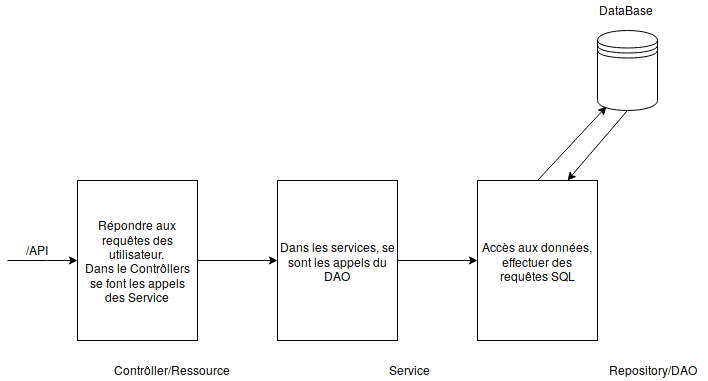
\includegraphics[width=1\textwidth]{diagrammes/ArchitectureProjet.png}
  		\caption{Arichtecture Back-end d'une application web}
	\end{figure}

\subsubsection{Front-end}
Le Front-end est la partie visible par les utilisateurs des applications web. Elle comprend l'interface graphique par laquelle nos utilisateurs vont interagir avec 
le reste du système (Back-end).


Le Front-end des applications web du rectorats sont développées en plusieurs langages. La plupart de ces applications  sont codées avec le triplet HTML,CSS \& JavaScript. Tandis que ces derniers mois, l'équipe informatique commence à intégrer le langage React.js  afin de monter en compétences et découvrir des nouveaux langages plus récents. 

\textbf{HTML:} HTML est une technologie et un standard qui permet d'afficher le contenu d'une application sur le web. Le langage reprend la syntaxe de XML,c'est-à-dire, une imbrication de balise/élément/tag les uns dans les autres. \newline
\newline
\textbf{CSS:} CSS, est une technologie complémentaire à HTML, c'est elle qui va permettre d'ajouter des couleurs, des ombres, de mettre en forme le texte, de positionner les blocs, etc. Elle sert à mettre en forme une page web. \newline
\newline
\textbf{JavaScript:} JavaScript, au contraire de HTML et CSS, n'est pas un langage de présentation mais de programmation, qui plus est, objet orienté prototype. Il permet de rendre plus dynamique une application web grâce à la manipulation de l'API DOM (Document Object Model) et de l'AJAX (Asynchronous JavaScript And XML).\newline
\newline
\textbf{React:} Le défaut de JavaScript, mais qui est aussi sa force, est sa grande flexibilité (typage dynamique, première ordre, point virgule optionnel...). On peut donc arriver très facilement à un code illisible et non maintenable. Le framework React apporte beaucoup de solutions à ces problèmes, avec sa façon de manipuler la DOM (via un moteur de template), l'utilisation de TypeScript (une amélioration du JavaScript par Microsoft.De plus, il est très facile de générer un environnement React pour un projet. C'est pour ces raisons que l'équipe informatique du rectorat commence à prendre en main ce Langage et l’intégrer dans les nouveaux projets et les nouvelles applications web. 

\begin{figure}[H]
	\centering
 		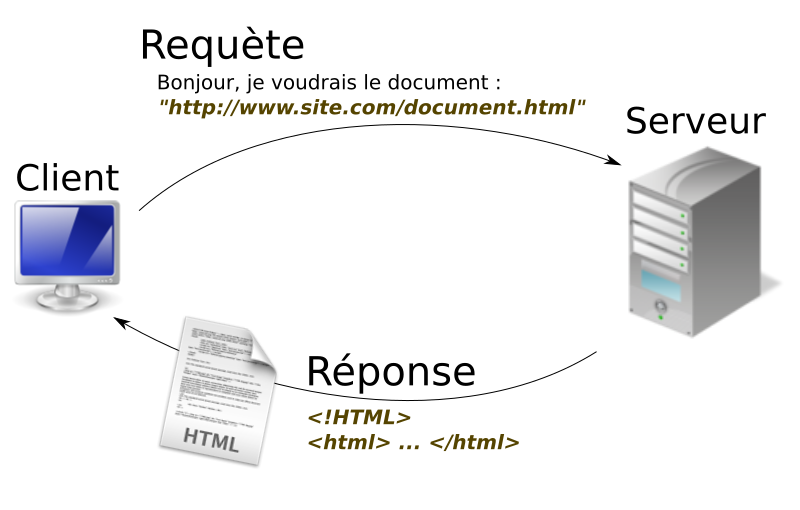
\includegraphics[width=1\textwidth]{diagrammes/schema-serveur.png} 
  		\caption{Application Web classique}
	\end{figure}

\subsection{Méthodes de travail}
\subsubsection{Méthodologie agile}

Les équipes informatiques du rectorat fonctionnent en méthodologie agile, chaque équipe effectue un Daily afin que chaque personne puisse présenter sur quoi elle a travaillé la veille et sur quoi elle compte continuer le jour même. Dans mon cas, j'étais le seul développeur dans mon projet, je faisais un Daily tout les jours avec mes maîtres d'alternances pour que je puisse dire sur quoi je travaillais et leurs poser des questions en cas de blocages. 

\subsubsection{Communication}

Pour communiquer, l'équipe informatique utilise l'outil de messagerie instantané Rocket.Chat. Il permet de créer différents
channels pour chaque équipe, des channels de veille ont été également crées pour de la veille technologies.

Nous utilisons aussi l'outil Calendar (un outil développer par Oracle) qui permet d’organiser les réunions.  

\subsubsection{Dockerisation}

Le logiciel Docker permet de créer, déployer et exécuter des conteneurs de manière efficace. Un conteneur enveloppe l’application d’un logiciel dans une boîte invisible avec tout ce dont il a besoin pour s’exécuter. Cela comprend le
système d’exploitation, le code de l’application, le runtime, les outils système et les librairies. Les conteneurs Docker sont construits à partir des images Docker.

Ils sont légers, portables et permettent aux développeurs de créer, déployer et exécuter efficacement des applications distribuées. En outre, ils permettent à une application d’être empaquetée et déplacée facilement, augmentant ainsi la simplicité d’une infrastructure.

\subsubsection{Versionning}

L'équipe informatique utilise Git sur la plateforme Gitlab hébergé par la Forge comme gestionnaire de versions. 


\section{Objectifs et missions de l'alternance}

\subsection{Objectif du projet}

Au sein du rectorat, le pôle DINAMO se charge de réaliser les applications web métiers et autres. L'équipe informatique utilise différentes façons pour documenter leur applications. La plupart du temps elle utilise une documentation écrite (Manuel Utilisateur), une chose qui ne rend pas facile aux utilisateurs d’interagir avec l'application et comprendre la documentation. 


C'est pour cette raison que Monsieur JOSSO Clément,le product Owner du projet(PO), a voulu mettre en œuvre une documentation interactive dans l'application métier Solycee afin de permettre aux utilisateurs de l'application de se auto-documenter et interagir directement avec la page web. Nous avons utilisé un outil nommé BootstrapTour pour réaliser cette documentation. 

Le but final du projet est de permettre aux administrateurs d'être autonomes et de pouvoir rajouter ou modifier les tours ainsi que leurs  étapes dans leurs applications. Nous avons donc crée un web service(AppTour) où sont sauvegardé tous les tours et leurs étapes.

\subsection{Présentation de Bootstrap Tour : Une visite guidée interactive}
 
Bootstrap tour est une petite librairie JavaScript permettant de présenter de façon assez simple l’application, l’avantage, comme pour toutes les librairies en fait, c’est qu’il y a déjà des bouts de fonctionnalités toutes faites, ce qui évite de réimplémenter le code. Bootstrap tour est une implémentation qui sert à créer une visite guidée pour une application.

Le bénéfice de l'utilisation de Bootstrap tour est immédiat pour les utilisateurs car elle présente les fonctionnalités de la page directement sur l'écran soit en lançant la documentation  dés l'ouverture de la page ou en appuyant sur un bouton pour déclencher cette documentation.

\subsection{Solycee}

Solycee est une application métier créée par le rectorat et destinée à la gestion des offres et demandes de stages. Elle permet aux collèges et aux lycées d'inscrire leurs élèves aux mini-stages proposés par les lycées.  

L'application serveur est réalisé en Java avec l'utilisation des composants du framework Spring.L'interface est codé avec le triplet HTML,CSS \& Javascript en intégrant du Thymeleaf pour le traitement des vues.  

\subsubsection{Aspect technique}

Le projet est implémenté selon le patron de conception MVC et réalisé avec plusieurs technologies, la plupart de ces dernières sont open-source.L'application est implémenté avec un back-end et un Front-end.

Le back-end a été implémenté avec le framework Spring et le langage Java. Le coté interface (Front-end) a été réalisé avec le moteurs de templâte Thymeleaf. 

Voici maintenant une présentation plus précise sur les principaux outils utilisés:\newline

\textbf{Spring:}  Spring est un framework libre pour construire et définir l'infrastructure d'une application java dont il facilite le développement et les tests.\newline

\begin{itemize}
	\item \textbf{Spring MVC} : Spring MVC est un framwork qui permet d’implémenter des applications selon le design pattern MVC. Donc, comme tous autre MVC framework, Spring MVC se base sur le principe décrit par le schéma ci-dessous :\newline
	

\begin{figure}[H]
	\centering
 		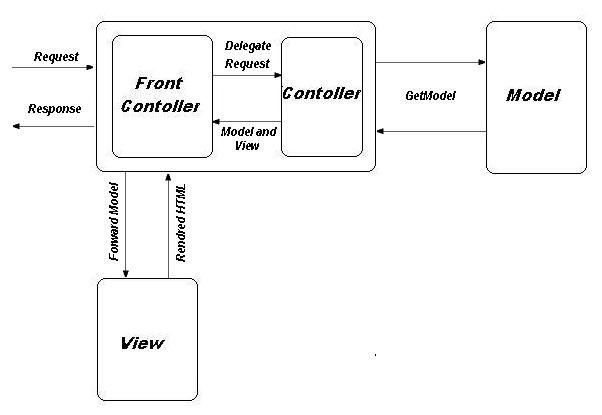
\includegraphics[width=1\textwidth]{diagrammes/mvc.jpg} 
  		\caption{Schéma du patron de conception MVC}
	\end{figure}
	
	\item \textbf{Spring Security }: Spring Security est un Framework de sécurité léger qui fournit une authentification et un support d’autorisation afin de sécuriser les applications Spring.\newline
\end{itemize} 

\textbf{Maven:} Maven est un outil de construction de projets (build) open source développé par la fondation Apache, initialement pour les besoins du projet Jakarta Turbine. Il permet de faciliter et d'automatiser certaines tâches de la gestion d'un projet Java.\newline

\textbf{Thymeleaf:} Thymeleaf est un  Java XML/XHTML/HTML5 Template Engine qui peut travailler à la fois dans des environnements Web (Servlet) et celui de non Web. Il est mieux adapté pour diffuser XHTML/HTML5 sur View (View Layer) des applications Web basées sur MVC. Mais il peut traiter n'importe quel fichier XML même dans les environnements hors ligne. Il fournit une intégration complète de Spring Framework. 

\subsubsection{Travail réalisé}

Dans le projet Solycee, j'ai principalement travaillé sur la partie Front-end. J'ai réalisé plusieurs tâches soit en rajoutant des nouvelles vue et des nouveaux composants dans les pages web et/ou en rajoutant des nouvelles fonctionnalités sur les composants existant. Voici une présentation plus précises de toutes les tâches réalisées: 

\begin{itemize}
\item Rajout d'une modale pour prévenir les utilisateurs de la présence d'un bouton aide pour déclencher la documentation interactif.

\begin{figure}[H]
	\centering
 		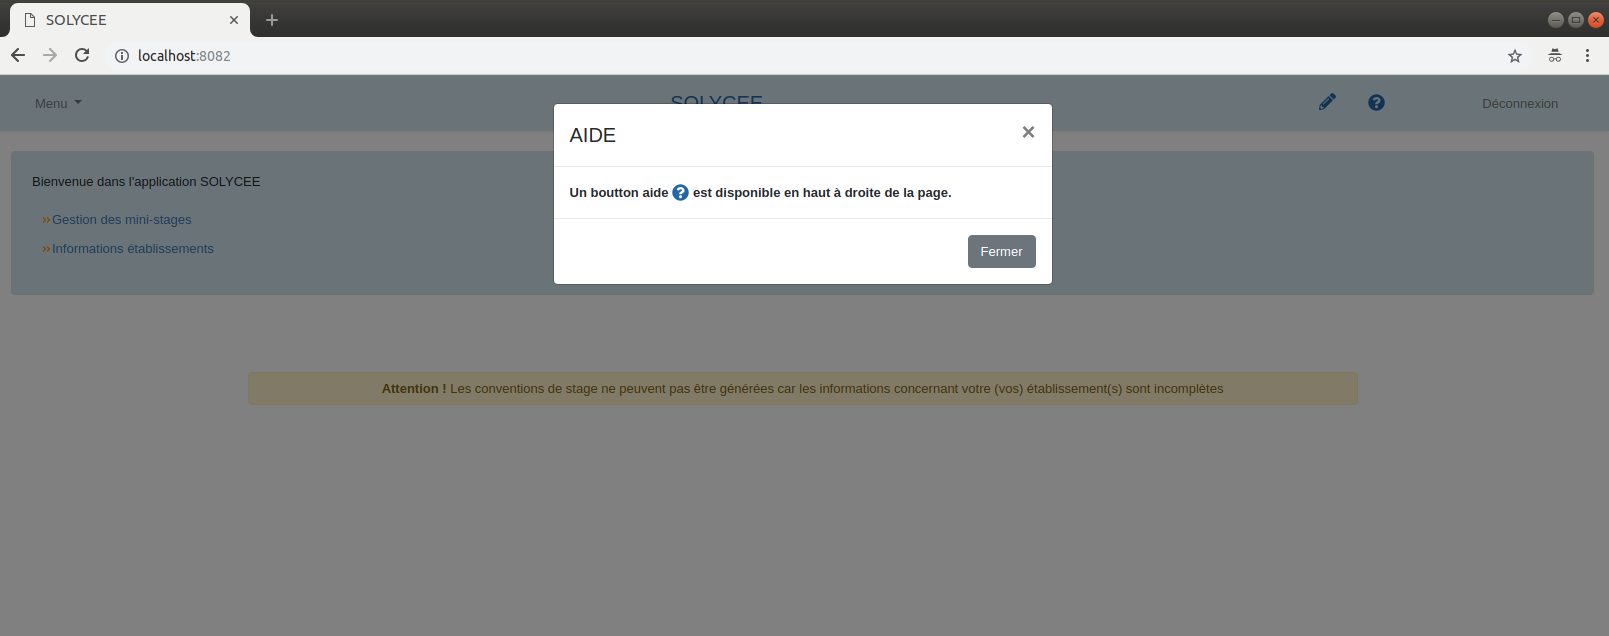
\includegraphics[width=1\textwidth]{diagrammes/aide_modal.png}
  		\caption{Image page d'accueil Solycee}
	\end{figure}
   
\item Rajout du Bootstrap Tour : Il s'agit de l'ajout d'un bouton 
\includegraphics[width=5mm,scale=0.5]{diagrammes/Bouton_aideDispo.png} sur toutes les pages web de l'application. En appuyant dessus ça déclenche les pop-ups  de Bootstrap tour (Les étapes du tour sur la page web), une étape se représente avec 3 champs: Element (élément cliqué, Titre (titre de l'étape) \& Content (Description de l'étape). Dans le cas où il n'existe pas de tour sur la page web, le bouton affiché est gris et titré par une phrase "Aide non disponible pour cette page" 
\includegraphics[width=7mm,scale=0.5]{diagrammes/Bouton_aideNonDispo.png}  

\begin{figure}[H]
	\centering
 		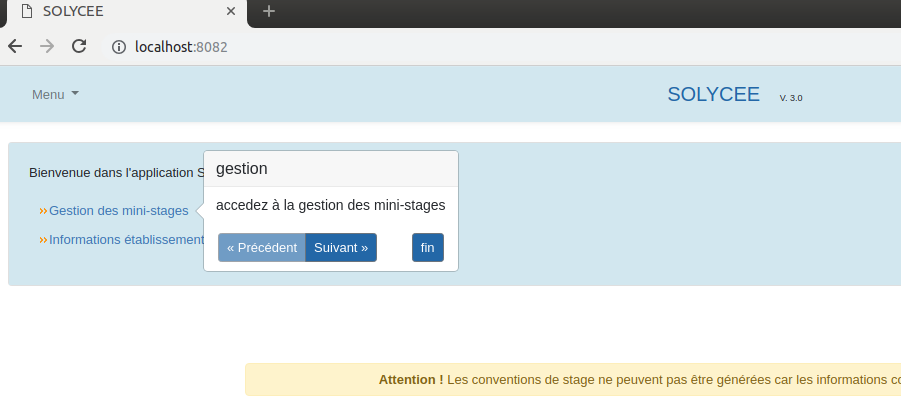
\includegraphics[width=1\textwidth]{diagrammes/exemple_Tour.png} 
  		\caption{Exemple d'une étape de Bootstrap Tour}
	\end{figure}

\item Récupérer le tour d'une page web avec ses étapes: Pour chaque page web de solycee, l'application récupère le tour de cette dernière avec ses étapes en lançant une requête à l'API AppTour. Cette requête (FindTourWithLibelleAplicationAndIdHtmlPage) renvois un json avec toutes les étapes en cas de la présence du tour dans la base. En cas où le tour n'existe pas et la requête renvoi une réponse 404 (Not found), nous mettons le bouton d'aide en gris et il devient non cliquable. 

\begin{figure}[H]
	\centering
 		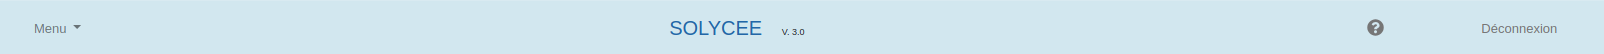
\includegraphics[width=1\textwidth]{diagrammes/aideNonDispo.png} 
  		\caption{Pas de tour disponible dans ce page Web }
	\end{figure}
    

\item Mode édition pour les Administrateurs : En appuyant sur le bouton  
\includegraphics[width=5mm,scale=0.5]{diagrammes/Bouton_modeEdition.png}, les administrateurs  de l'application passent en mode édition. Il s'agit d'un mode avec la même interface graphique mais les composants et les boutons de cette interface ne réagissent plus de la même façon(Le fonctionnement de ces composant se désactive). En appuyant sur un des composant de la page, il y a une modale qui s'affiche pour permettre aux admins de rajouter des étapes de leur tour dans cette page Web.  Nous affichons aussi un champs sur l'interface Web pour afin de prévenir les admins qu'ils ont passé en mode édition.

 \begin{figure}[H]
	\centering
 		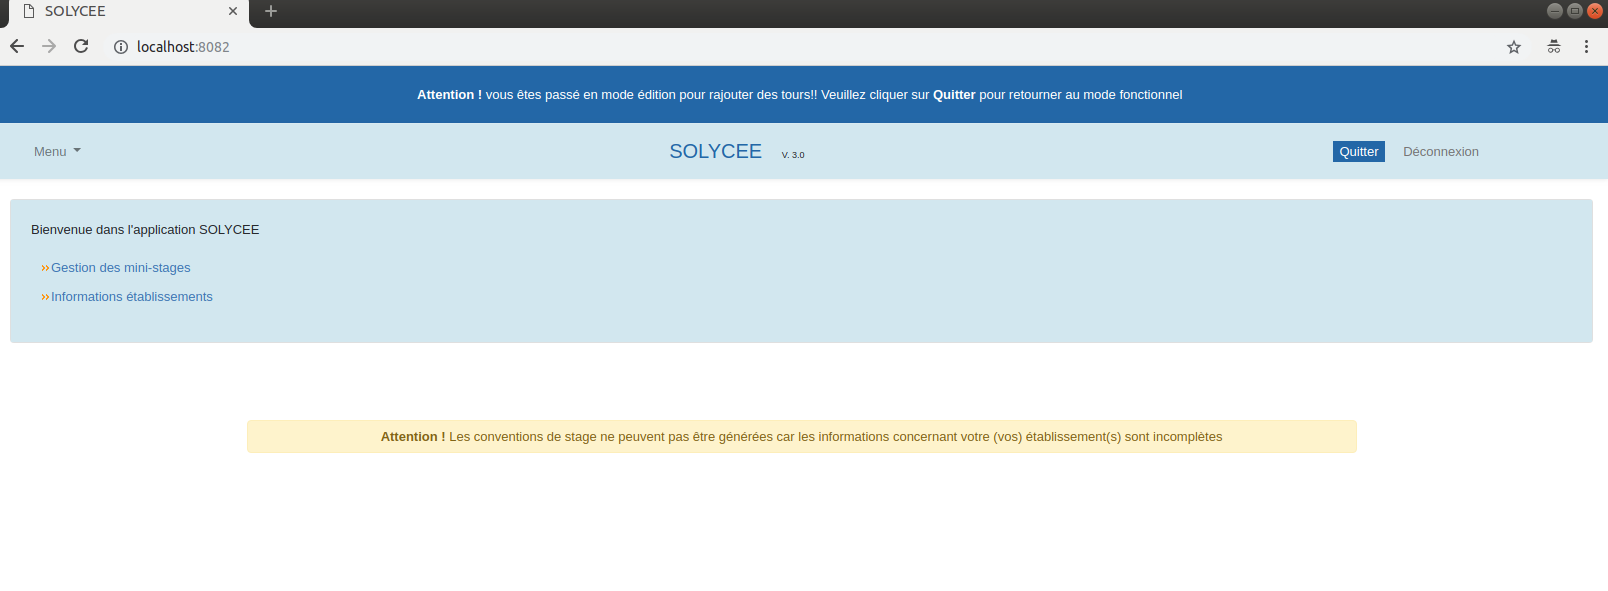
\includegraphics[width=1\textwidth]{diagrammes/mode_edition.png} 
  		\caption{Page d'accueil en mode édition}
	\end{figure}

\item Permettre seuls aux administrateurs de voir le bouton qui permet de passer en mode édition. En se connectant à l'application, nous récupérons le nom complet de l'utilisateur connecté et nous envoyons une requête à l'API AppTour pour voir si l'utilisateur est administrateur. Si la requête renvoie le json de l’utilisateur nous affichons le bouton, dans le cas inverse le bouton sera pas affiché. \newline 

\item Rajouter ou modifier les étapes :Quand les administrateurs se mettent en mode édition et en appuyant sur les composant de la page web(Boutons, liens ou autres), une modale s'affiche afin de permettre aux administrateurs de rajouter une étape du tour dans le cas où aucune étape existe pour le composant appuyé ou modifier l'étape si elle existe. 
La récupération de l'étape de chaque composant se fait par un appel à l'API AppTour (FindStepByElementandIdTour), dans le cas où l'étape existe, nous remplissons les champs de la modale avec les données récupérées par la requêtes(Title \& content). Dans le cas inverse, nous laissons les champs vide afin que les administrateurs remplissent les données qui veulent stocker dans la base AppTour.

Il existe un bouton valider dans la modal qui  permet soit de rajouter la nouvelle méthode avec la méthode POST si elle n'existe pas ou sinon modifier les éléments de l'étape avec une méthode PUT. 
\end{itemize}

\subsection{AppTour}   

Au début du projet, j'ai commencé par manipuler BootstrapTour sur l'application Solycee en rajoutant le code de la librairie dans le front de Solycee (code en javascript avec les étapes souhaités). Bootstrap tour permet d'afficher l'étape du tour et aussi passer à l'étape suivante ou précédente ainsi que arrêter le tour avec le bouton "Fin".

Cette manipulation est simple et efficace pour un développeur pour rajouter des tours et leurs étapes afin de faire une visite d'application. Il suffit juste de manipuler le code Javascript. Chose qui n'est pas facile pour d'autres personnes ou les administrateurs de l'application.

AppTour est un web service qui permet aux administrateurs des applications du rectorat d'être plus autonome afin qu'il puissent rajouter ou/et modifier des étapes sans aller chercher dans le code. Tous les tours et les étapes de toutes les applications où nous souhaitons mettre du Bootstrap tour seront sauvegardés dans le web service AppTour.   

API Apptour est une application Sring Boot codé en langage Kotlin. Le but de cette application est d’implémenter plusieurs  services afin de permettre aux administrateurs des autres applications de rajouter et modifier les étapes. 


\subsubsection{Aspect technique}
 
 Le projet AppTour était initialiser par l'alternant de l'année dernière. j'ai commencé par la relecture du code et la compréhension de l'existant. L'application a été implémenté en Kotlin qui est un langage de programmation orienté objet et fonctionnel, avec un typage statique qui permet de compiler pour la machine virtuelle Java et JavaScript et Spring boot qui est un framework utilisé afin de faciliter la configuration d'un projet Spring et de réduire le temps alloué au démarrage d'un projet. plusieurs autres technologies était utilisées dans ce projet : 
 
\begin{itemize}
\item Maven :  Est un outil de gestion et d'automatisation de production des projets logiciels Java en général et Java EE en particulier. Il est utilisé pour automatiser l'intégration continue lors d'un développement de logiciel.

\item JUnit : Pendant mon développement de l'API AppTour, j'ai utilisé la méthode du TDD(Test Driven Development),le développement piloté par les tests. j'ai utilisé le framework JUnit pour implémenter les tests unitaires afin d'assurer la maintenance et l'efficacité de l’application.

\item Git : Est un logiciel de gestion de versions décentralisé. Il permet de sauvegarder les fichiers en gardant la chronologie de chaque sauvegarde.

\item L'API AppTour a été réalisé de la même manière que les autres applications du rectorat. Il existe plusieurs couches. Une couche service pour implémenter tous les services dont nous avons besoin, une couche controller pour construire l'API utilisée par le Front Solycee et qui sera utilisée par d'autres applications dans le futur, il existe d'autres couches afin de créer une application similaire aux autres applis du rectorat.

\end{itemize}

\subsubsection{Travail réalisé}


\end{document}
